%-----------------------------------
%   PROTOCOLO DE ENRUTAMIENTO
%-----------------------------------
\chapter{Protocolo de enrutamiento}

\label{ch:protocolo_de_enrutamiento}

El protocolo de enrutamiento propuesto permite que dispositivos móviles puedan
comunicarse entre sí mediante el servicio de red proporcionado por la VANET.
Existen dos tipos de dispositivos que forman parte de la red. Los
\textit{hosts} son los dispositivos que ejecutan las aplicaicones que requieren
enviar información a otros. Los vehículos son los que se encargan de realizar
el enrutamiento de paquetes de un \textit{host} a otro.

Una vez que los vehículos tienen asignada una dirección IP, pueden comunicarse
entre sí a través de la red. Cuando un vehículo recibe un paquete, necesita
consultar su tabla de enrutamiento para saber hacia dónde lo debe retransmitir
para que llegue a su destino, como se menciona en la sección
\ref{sec:tablas_de_enrutamiento}. Sin embargo, se necesita un protocolo de
enrutamiento que se encargue de llenar la tabla.

Los vehículos tienen que compartir mensajes entre ellos con información que les
ayude a determinar hacia dónde tiene que enviar cada paquete de información. El
protocolo propuesto es basado en la posición, por lo que cada vehículo debe
compartir información, entre otras cosas, sobre su ubicación.

En este capítulo, se describe el funcionamiento del protocolo de enrutamiento
propuesto, es decir, cómo se determinan las rutas y los tipos de mensajes que
los vehículos se compartirán, además de cómo deben procesar estos mensajes para
llenar las tablas de enrutamiento.

%-----------------------------------
%   CRITERIOS GENERALES DE RETRANSMISIÓN DE PAQUETES
%-----------------------------------
\section{Criterios generales de retransmisión de paquetes}

\label{sec:criterios_generales_retransmision_paquetes}

Los protocolos basados en la posición, como se mencionó en la sección
\ref{sec:enrutamiento_basado_en_la_posicion}, consideran la ubicación de los
dispositivos para hacer decisiones sobre el enrutamiento. Por ejemplo, en el
protocolo GPSR, discutido en la sección \ref{subsubsec:retransmision_voraz},
cada nodo únicamente considera su ubicación, la del destinatario y las de los
vecinos, y selecciona el más cercano al destino. Sin embargo, en un ambiente
urbano es frecuente que existan obstáculos, principalmente edificios, que
bloqueen las transmisiones. Este tipo de transmisiones se conocen como
transmisiones sin \textbf{línea de visión}. La figura
\ref{fig:transmision_sin_linea_de_vision} muestra una transmisión en la que un
edificio se encuentra entre los vehículos A y B.

\begin{figure}[th]
\centering
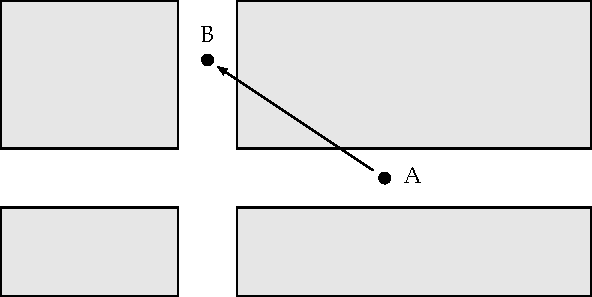
\includegraphics{transmision_sin_linea_de_vision}
\decoRule
\caption[Transmisión sin línea de visión]{Transmisión sin línea de visión.}
\label{fig:transmision_sin_linea_de_vision}
\end{figure}

Una transmisión sin línea de visión tiene más probabilidad de resultar en un
paquete perdido. Cuando un paquete se pierde, en la mayoría de los casos, debe
ser retransmitido. La pérdida de paquetes se debe evitar, ya que, mientras más
paquetes se pierdan y deban ser retransmitidos, el canal de comunicación tiende
a usarse más para retransmitir paquetes perdidos y no para transmitir paquetes
nuevos.

Para reducir la pérdida de paquetes, el protocolo prupuesto busca que las
transmisiones entre los vehículos tengan línea de visión. Por ejemplo, en la
figura \ref{fig:transmision_misma_calle}, el vehículo A tiene un paquete cuya
ruta demanda que pase por el vehículo C. Para esto, hay dos opciones para
seleccionar el siguiente salto: el vehículo B y el vehículo C. Si se selecciona
directamente el vehículo C, la transmisión encontraría un edificio en el
camino. Por esto, se selecciona el vehículo B, que circula sobre la misma
calle, como siguiente salto, y este retransmite el paquete al vehículo C.

\begin{figure}[th]
\centering
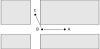
\includegraphics{transmision_misma_calle}
\decoRule
\caption[Transmisiones con línea de visión]{Transmisiones con línea de visión.}
\label{fig:transmision_misma_calle}
\end{figure}

Para lograr esto, cada vehículo debe poder saber qué vehículos se encuentran
circulando sobre su misma calle. Se puede considerar que, de cierta forma, los
paquetes recorren las calles a través de los vehículos. En la figura
\ref{fig:paquete_recorre_calle_1}, se muestra un paquete que es retransmitido
entre varios vehículos. En la figura \ref{fig:paquete_recorre_calle_2}, se
muestra el mismo escenario, pero se interpreta como el paquete recorriendo las
calles para moverse de un cruce vial a otro.

\begin{figure}[th]
\centering
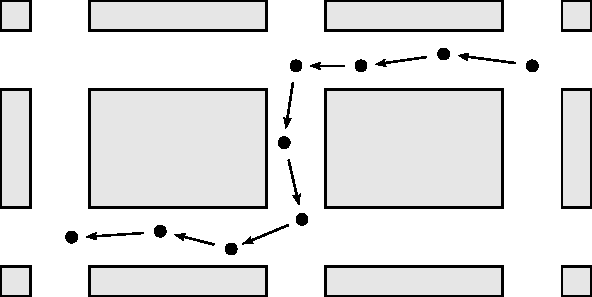
\includegraphics{paquete_recorre_calle_1}
\decoRule
\caption[Paquete siendo retransmitido entr vehículos]{Paquete siendo
retransmitido entre vehículos.}
\label{fig:paquete_recorre_calle_1}
\end{figure}

\begin{figure}[th]
\centering
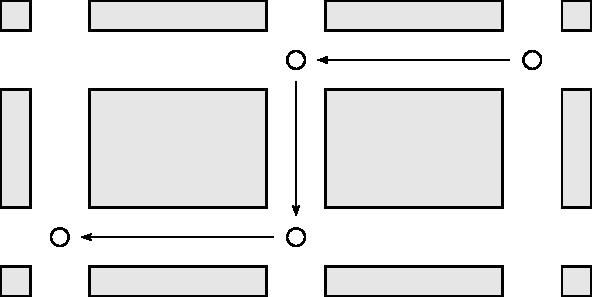
\includegraphics{paquete_recorre_calle_2}
\decoRule
\caption[Paquete recorriendo las calles]{Paquete recorriendo las calles.}
\label{fig:paquete_recorre_calle_2}
\end{figure}

Cuando un paquete llega al final de un segmento de calle y se encuentra en un
cruce vial, el vehículo portador debe determinar hacia qué calle debe seguir el
paquete para llegar a su destino, y seleccionar un vehículo que circule sobre
esa calle. En la figura \ref{fig:decision_cruce}, el vehículo B recibe un
paquete del vehículo A, y puede elegir entre tres calles para retransmitir el
paquete.

\begin{figure}[th!]
\centering
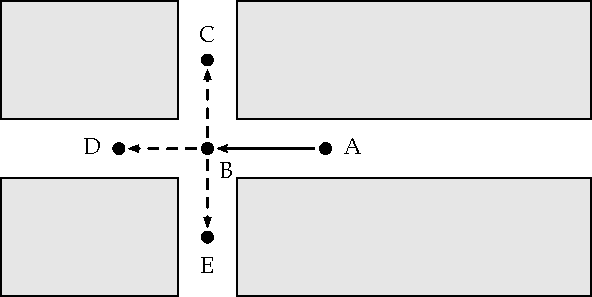
\includegraphics{decision_cruce}
\decoRule
\caption[Decisión de enrutamiento en cruce vial]{Decisión de enrutamiento en
cruce vial.}
\label{fig:decision_cruce}
\end{figure}

Para tomar este tipo de decisiones, se necesita que cada vehículo cuente con
información sobre la topología vial que le ayude a determinar cuál es la mejor
ruta. A continuación, se presenta cómo se estructura esta información y cómo se
utiliza durante el proceso de enrutamiento.

%-----------------------------------
%   GRAFO VIAL
%-----------------------------------
\section{Grafo vial}

\label{sec:grafo_vial}

En el protocolo propuesto, hay dos maneras de analizar el enrutamiento:
enrutamiento de red y enrutamiento vial. En el \keyword{enrutamiento de red},
se consideran los vehículos que conforman la ruta desde el origen hasta el
destino, y forman una \keyword{ruta de red}. En el \keyword{enrutamiento vial},
se consideran las calles que recorre un paquete para llegar a su destino, que
componen una \keyword{ruta vial}.

Para determinar una ruta vial, se define un grafo que represente la topología
vial para cada subred Geohash, denominado \keyword{grafo vial}, o \keyword{red
vial}. Se trata de un grafo no dirigido $\mathbf{G}=(\mathbf{V},\mathbf{E})$,
en el que $\mathbf{V}$ es el conjunto de vértices, que representan los cruces
viales, y $\mathbf{E}$ es el conjunto de aristas, que representan los segmentos
de las calles. La figura \ref{fig:grafo_vial_1} muestra el mapa de una región
Geohash, y su correspondiente grafo vial se muestra en la figura
\ref{fig:grafo_vial_2}.

\begin{figure}[th!]
\centering
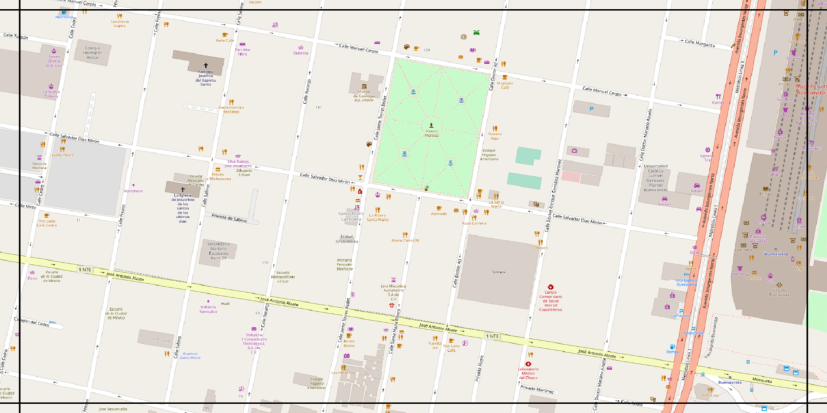
\includegraphics{grafo_vial_1} 
\decoRule
\caption[Región Geohash 9g3qxs]{Región Geohash 9g3qxs.}
\label{fig:grafo_vial_1}
\end{figure}

\begin{figure}[th!]
\centering
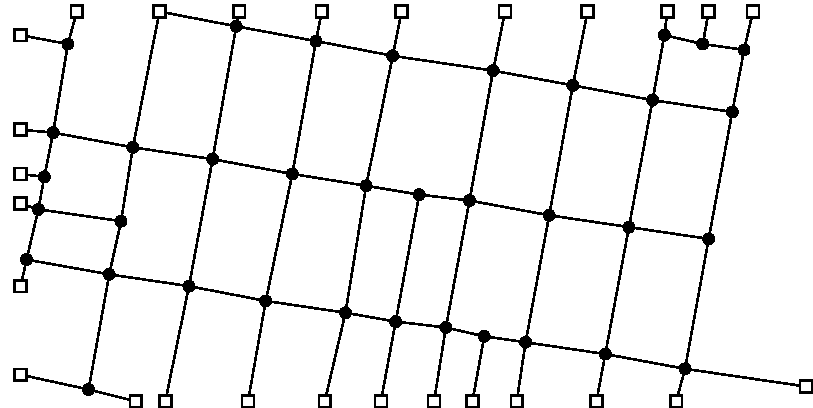
\includegraphics{grafo_vial_2} 
\decoRule
\caption[Grafo vial de la región Geohash 9g3qxs]{Grafo vial de la región
Geohash 9g3qxs.}
\label{fig:grafo_vial_2}
\end{figure}

Un grafo vial no pretende ser una representación fiel de la topología vial,
sino que se usa para determinar una ruta vial. Cada arista representa todos los
carriles que corresponden al segmento de calle que representa. Por otro lado,
cada vértice representa una ubicación en la que un vehículo puede transmitir
con posible línea de visión un paquete hacia los segmentos de calles que ahí
insiden. Por esta razón, los vértices son los puntos en los que los vehículos
toman decisiones de enrutamiento importantes.

En la sección \ref{sec:cambio_subred}, se usó el concepto de región
\textit{gateway} para explicar cómo un vehículo se autocofigura para unirse a
la subred adyacente y compartir paquetes entre ambas subredes. Sin emabargo, en
la realidad se utilizan los vértices del borde de un grafo vial para realizar
esta función, por lo que se denominan \keyword{vértices \textit{gateway}}, y se
muestran como cuadrados en la figura \ref{fig:grafo_vial_2}. De manera
similar, las aristas que tienen un vértice \textit{gateway} se denominan
\keyword{aristas \textit{gateway}}. Cuando un vehículo circula por una arista
\textit{gateway}, este asume que entró a la región \textit{gateway}, y realiza
el procedimiento descrito en la sección \ref{sec:cambio_subred}.

%-----------------------------------
%   ENRUTAMIENTO VIAL
%-----------------------------------
\section{Enrutamiento vial}

\label{sec:enrutamiento_vial}

Una \keyword{ruta vial} indica qué calles recorre un paquete para llegar a su
destino, y los vehículos que permiten que un paquete siga una ruta vial forman
una \keyword{ruta de red}. Debido a que los vehículos están en constante
movimiento, dos paquetes que sigan la misma ruta vial no necesariamente
seguirán la misma ruta de red.

Cuando el remitente y el destinatario se encuentran dentro de la misma región
Geohash, y, por lo tanto, pertenecen a la misma subred, se lleva a cabo lo que
se denomina \keyword{enrutamiento intrarregión}. En este caso, únicamente se
necesita conocer las calles que el paquete debe recorrer, que forman una
\keyword{ruta intrarregión}. Esto se traduce a determinar una ruta entre dos
vértices del grafo vial.

En la figura \ref{fig:enrutamiento_intrarregion}, un paquete debe llegar del
vehículo $V_1$ al vehículo $V_2$. Una ruta intrarregión que le permite al
paquete llegar al vehículo $V_2$ se muestra en la figura, y se forma por la
seuencia de vértices $h \rightarrow g \rightarrow f \rightarrow j$.

\begin{figure}[th!]
\centering
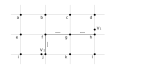
\includegraphics{enrutamiento_intrarregion}
\decoRule
\caption[Enrutamiento intrarregión]{Enrutamiento intrarregión.}
\label{fig:enrutamiento_intrarregion}
\end{figure}

Cuando el remitente y el destinatario se encuentran en regiones Geohash
diferentes, se debe realizar lo que se llama \textbf{enrutamiento interregión}.
Este consiste en determinar de qué subred a qué subred debe viajar un paquete
para llegar a la subred donde se encuentra el destino, lo que se denomina
\textbf{ruta interregión}. Cuando un paquete entra a una subred a través de un
vértice \textit{gateway}, se determina una ruta intrarregión que le permita
llegar a un vértice \textit{gateway} por el que pueda llegar a la siguiente
subred.

La figura \ref{fig:enrutamiento_interregion} muestra una ruta interregión que
indica por qué subredes debe pasar un paquete para llegar del vehículo $V_1$
al vehículo $V_2$. La ruta interregión se forma por las subredes 9g3qxm
$\rightarrow$ 9g3qxt $\rightarrow$ 9g3qxs $\rightarrow$ 9g3qxu.

\begin{figure}[th!]
\centering
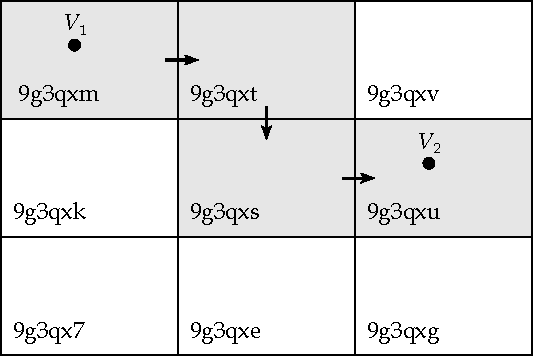
\includegraphics{enrutamiento_interregion}
\decoRule
\caption[Enrutamiento interregión]{Enrutamiento interregión.}
\label{fig:enrutamiento_interregion}
\end{figure}

%-----------------------------------
%   UBICACIÓN VIAL
%-----------------------------------
\section{Ubicación vial}

\label{sec:ubicacion_vial}

Los vehículos pueden conocer su ubicación en coordenadas geográficas (latitud y
longitud), así como la dirección y velocidad de su movimiento. No obstante,
para proporcionar información más útil a sus vecinos, cada vehículo también
necesita conocer su ubicación en el grafo vial de la subred donde se encuentra.
La \keyword{ubicación vial} de un vehículo indica en qué arista circula y su
distancia uno de los vértices de esta.

\begin{figure}[th!]
\centering
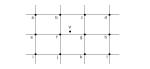
\includegraphics{ubicacion_vial_1} 
\decoRule
\caption[Vehículo en una red vial]{Vehículo en una red vial.}
\label{fig:ubicacion_vial_1}
\end{figure}

Las coordenadas de los vértices son conocidas, pero no se conoce el ancho de
cada calle, sino que se representan como segmentos de recta entre pares de
vértices. Es por esto que la ubicación del vehículo no cae exactamente sobre la
arista, sino en un punto cercano a esta. En la figura
\ref{fig:ubicacion_vial_1}, se muestra una red vial en la que hay un vehículo
en el puntio $V$.

\begin{figure}[th!]
\centering
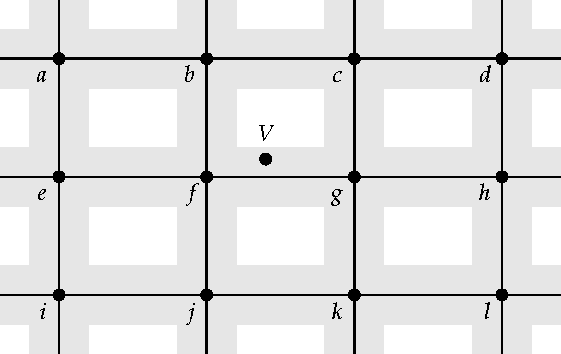
\includegraphics{ubicacion_vial_2} 
\decoRule
\caption[Dominio de las aristas en una red vial]{Dominio de las aristas en una
red vial.}
\label{fig:ubicacion_vial_2}
\end{figure}

La ubicación de un vehículo difícilmente cae exactamente sobre la arista
por donde circula, como se mencionó anteriormente. Por esta razón, se
consideta una región alrededor de la arista, denominada \keyword{dominio de la
arista}.  El dominio de una arista se delimita por dos líneas paralelas a la
arista, una a cada lado. En la figura \ref{fig:ubicacion_vial_2} se muestra el
dominio de cada arista, y se observa que el vehículo se encuentra dentro del
dominio de la arista $\{f,g\}$.

Si un vehículo se encuentra dentro del dominio de una arista, es posible que se
encuentre circulando por esta. Sin embargo, esta no es la única condición que
se debe cumplir para considerar que esto es verdad. Además de esto, la
dirección de su velocidad debe coincidir con la dirección de la arista. Cada
arista tiene dos direcciones, llamadas \keyword{direcciones de la arista}, como
se muestra en la figura \ref{fig:direcciones_arista}. Cada dirección es un
ángulo acimutal que indica hacia dónde se encuentra un vértice de la arista
respecto al otro.

\begin{figure}[th!]
\centering
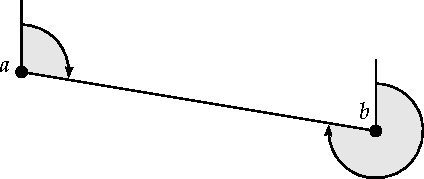
\includegraphics{direcciones_arista}
\decoRule
\caption[Direcciones de una arista]{Direcciones de una arista.}
\label{fig:direcciones_arista}
\end{figure}

Ya que cada vehículo es capaz de conocer la dirección de su movimiento, y las
direcciones de cada arista debido a que conoce la posición de sus vértices, se
puede determinar si estas coinciden. En la figura \ref{fig:ubicacion_vial_3} se
muestra que el vehículo se mueve en la misma dirección que la dirección del
vértice $g$ respecto al vértice $f$, y se encuentra dentro del dominio de la
arista $\{f,g\}$, por lo que se considera que está circulando sobre esa arista.

\begin{figure}[th!]
\centering
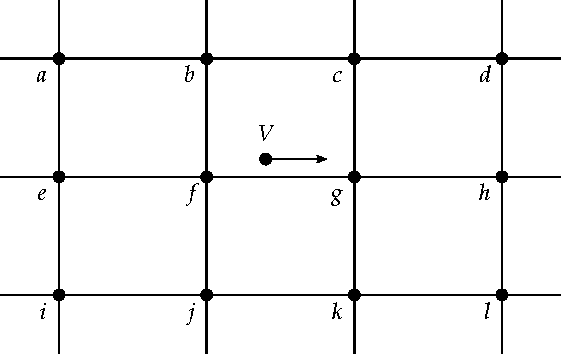
\includegraphics{ubicacion_vial_3} 
\decoRule
\caption[Dirección del movimiento de un vehículo en una red vial]{Dirección del
movimiento de un vehículo en una red vial.}
\label{fig:ubicacion_vial_3}
\end{figure}

Además de conocer en qué arista se encuentra circulando un vehículo, se
necesita saber en qué posición se encuentra circulando en dicha arista. Para
esto, se obtiene la proyección de la ubicación del vehículo en la arista y se
calcula su distancia a uno de los dos vértices, como se muestra en la figura
\ref{fig:ubicacion_vial_4}, donde se muestra la distancia al vértice $f$.

\begin{figure}[th!]
\centering
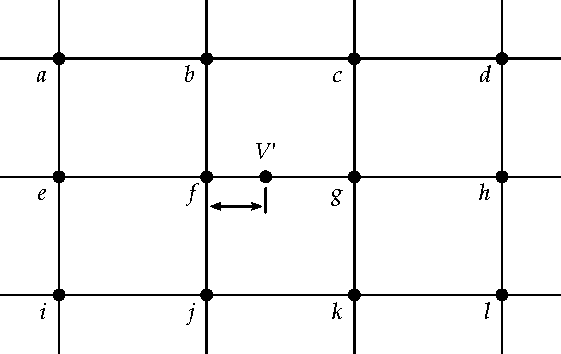
\includegraphics{ubicacion_vial_4} 
\decoRule
\caption[Posición de un vehículo en una red vial]{Posición de un vehículo en
una arista.}
\label{fig:ubicacion_vial_4}
\end{figure}

La ubicación vial de un vehículo consiste en los dos vértices de la arista
por la que circula y su posición en esta arista, es decir la distancia de su
proyección en la arista al primer vértice. Además, si su distancia a alguno de
los dos vértices de la arista es menor a un límite, cuyo valor se define por el
parámero RADIO\_CERCANIA\_VERTICE, se considera que \keyword{el vehículo se
encuentra en el vértice}.

%-----------------------------------
%   CABECERAS DE OPCIONDES DE SALTO POR SALTO
%-----------------------------------
\section{Cabecera de opciones de salto por salto}

\label{sec:cabecera_opciones}

Los paquetes deben incluir información que permita a los vehículos tomar
decisiones de enrutamiento. Las cabeceras de extensión sirven para incluir
información opcional adicional en un datagrama. La función de la
\keyword{cabecera de opciones de salto por salto} es contener información que
toods los enrutadores (vehículos en este caso) puedan revisar. Por esta razón,
esta cabecera se usa para incluir la información de enrutamiento en el paquete.
La figura \ref{fig:formato_datagrama_ipv6_cabecera} muestra la estructura del
datagrama IPv6 con la cabecera de opciones de salto por salto, y el formato de
esta cabecera se muestra en la figura
\ref{fig:formato_cabecera_salto_por_salto} \cite{RFC2460}.

\begin{figure}[th!]
\centering
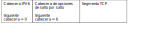
\includegraphics{formato_datagrama_ipv6_cabecera} 
\decoRule
\caption[Datagrama IPv6 con la cabecera de opciones de salto por
salto]{Datagrama IPv6 con la cabecera de opciones de salto por salto.}
\label{fig:formato_datagrama_ipv6_cabecera}
\end{figure}

\begin{figure}[th!]
\centering
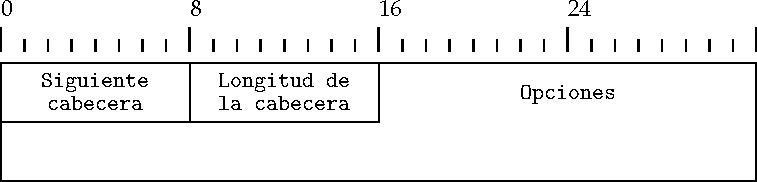
\includegraphics{formato_cabecera_salto_por_salto}
\decoRule
\caption[Formato de la cabecera de salto por salto]{Formato de la cabecera de
salto por salto.}
\label{fig:formato_cabecera_salto_por_salto}
\end{figure}

Los campos de la cabecera de opciones de salto por salto son los siguientes:

\keyword{Siguiente cabecera (8 bits)} -- Identifica el tipo de cabecera que
sigue después.

\keyword{Longitud de la cabecera (8 bits)} -- Longitud, en unidades de 8
octetos, de la cabecera de salto por salto, sin incluir los primeros 8 bytes.

\keyword{Opciones (longitud variable)} -- Secuencia de opciones que se procesan
en cada enrutador. Su longitud debe ser tal que la longitud total de la
cabecera de salto por salto sea un múltiplo entero de 8 octetos.

Las opciones se codifican con el formato tipo-longitud-valor (TLV), que se
muestra en la figura \ref{fig:formato_tlv}. Los campos de cada opción son los
siguientes \cite{RFC2460}:

\begin{figure}[th!]
\centering
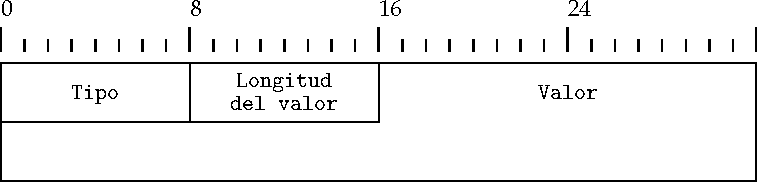
\includegraphics{formato_tlv}
\decoRule
\caption[Formato TLV]{Formato TLV.}
\label{fig:formato_tlv}
\end{figure}

\keyword{Tipo (8 bits)} -- Identificador del tipo de opción.

\keyword{Longitud del valor (8 bits)} -- Longitud en octetos del campo del
valor del dato.

\keyword{Valor (longitud variable)} -- Valor de la opción.

En el tipo de opción, los dos primeros bits indican qué hacer si la opción no
es reconocida, y el tercer bit indica si el valor del dato puede cambiar o no a
lo largo de la ruta.

%-----------------------------------
%   OPCIÓN DE UBICACIÓN DEL DESTINO
%-----------------------------------
\subsection{Opción de ubicación del destino}

\label{subsec:opcion_de_ubicacion_del_destino}

Para poder enrutar un paquete, el \textit{host} que lo origina agrega la
\keyword{opción de ubicación del destino} a la cabecera de opciones de salto
por salto. El formato de la opción de ubicación del destino se muestra en la
figura \ref{fig:formato_opcion_ubicacion_destino}, y contiene los siguientes
campos:

\begin{figure}[th!]
\centering
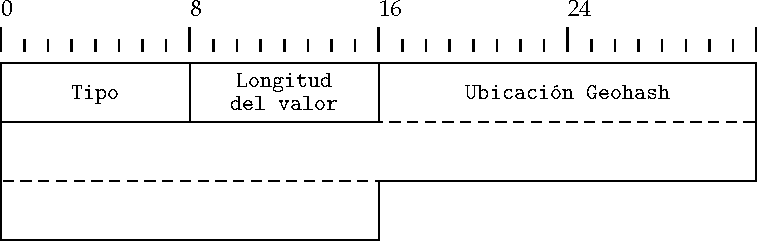
\includegraphics{formato_opcion_ubicacion_destino}
\decoRule
\caption[Formato de la opción de ubicación del destino]{Formato de la opción de
ubicación del destino.}
\label{fig:formato_opcion_ubicacion_destino}
\end{figure}

\keyword{Tipo (8 bits)} -- El tipo de la opción es 88, donde los primeros dos
bits indican que el paquete debe ser descartado si no se reconoce el tipo de
opción, y el tercer bit indica que el valor de la opción no cambia a lo largo
de la ruta.

\keyword{Longitud del valor (8 bits)} -- La longitud del valor es de 8 octetos.

\keyword{Ubicación Geohash (64 bits)} -- Ubicación Geohash de longitud 12 del
\textit{host} de destino.

%-----------------------------------
%   OPCIÓN DE UBICACIÓN VIAL DEL DESTINO
%-----------------------------------
\subsection{Opción de ubicación vial del destino}

\label{subsec:opcion_de_ubicacion_vial_del_destino}

Cuando un vehículo recibe un paquete, puede revisar la opción de ubicación del
destino para saber la ubicación geográfica a donde este tiene que llegar. Sin
embargo, para calcular una ruta vial, también se debe conocer la ubicación vial
destino.

Si un vehículo recibe un paquete cuyo destino se encuentra en la misma subred,
debe calcular la ubicación vial del destino y agregarla a la cabecera de
opciones con la \keyword{opción de ubicación vial del destino}. El formato de
este tipo de opción se muestra en la figura
\ref{fig:formato_opcion_ubicacion_vial_destino}, y contiene los siguientes
campos:

\begin{figure}[th!]
\centering
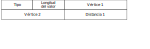
\includegraphics{formato_opcion_ubicacion_vial_destino}
\decoRule
\caption[Formato de la opción de ubicación vial del destino]{Formato de la
opción de ubicación vial del destino.}
\label{fig:formato_opcion_ubicacion_vial_destino}
\end{figure}

\keyword{Tipo (8 bits)} -- El tipo de la opción es 25, donde los primeros dos
bits indican que la opción se ignora si no se reconoce el tipo de opción, y el
tercer bit indica que el valor no cambia a lo largo de la ruta.

\keyword{Longitud del valor (8 bits)} -- La longitud del valor es de 6 octetos.

\keyword{Vértice 1 (16 bits)} -- Vértice 1 de la arista donde se ecuentra el
destino.

\keyword{Vértice 2 (16 bits)} -- Vértice 2 de la arista donde se ecuentra el
destino.

\keyword{Distancia 1 (16 bits)} -- Valor entero de la distancia en metros al
vértice 1.

Si un el destino un paquete se encuentra en una subred diferente a la subred en
la que se encuentra, no necesita llevar esta opción, ya que primero se debe
enrutar entre las subredes hasta llegar a la correspondiente. El primer
vehículo que recibe el paquete y se encuentra en la misma subred que el destino
se encarga de agregar esta opción.

%-----------------------------------
%   OPCIÓN DE VÉRTICES VISITADOS
%-----------------------------------
\subsection{Opción de vértices visitados}

\label{subsec:opcion_de_vertices_visitados}

Para evitar que un paquete pase más de una vez por el mismo vértice, debe
llevar un registro de los vértices por los que ha pasado. Estos se indican en
la \keyword{opción de vértices visitados}. El formato de esta opción se indica
en la figura \ref{fig:formato_opcion_vertices_visitados}, y contiene los
siguientes campos:

\begin{figure}[th!]
\centering
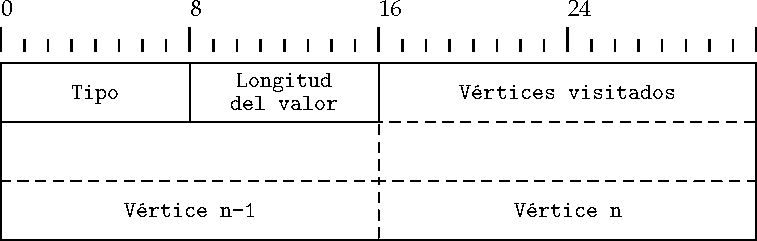
\includegraphics{formato_opcion_vertices_visitados}
\decoRule
\caption[Formato de la opción de vértices visitados]{Formato de la opción de
vértices visitados.}
\label{fig:formato_opcion_vertices_visitados}
\end{figure}

\keyword{Tipo (8 bits)} -- El tipo de la opción es 58, donde los primeros dos
bits indican que la opción se ignora si no se reconoce el tipo de opción, y el
tercer bit indica que el valor puede cambiar a lo largo de la ruta.

\keyword{Longitud del valor (8 bits)} -- La longitud del valor es variable.

\keyword{Vértices visitados (longitud variable)} -- Lista de vértices por los
que el paquete ha pasado. Cada vértice ocupa 2 octetos.

La opción de vértices visitados sólo es válida dentro de una subred. Cuando un
paquete pasa de una subred a otra, se elimina la opción de vértices visitados
de la cabecera y se agrega una nueva para los vértices de la siguiente subred.

%-----------------------------------
%   FORMATO DE LOS MENSAJES
%-----------------------------------
\section{Formato de los mensajes}

\label{sec:formato_mensajes}

Los tipos de mensajes que define el protocolo propuesto son
anuncio-\textit{host} (ANC-HOST), anuncio-vehículo (ANC-VEHIC),
\textit{ping}-vértice (PING), \textit{pong}-vértice (PONG) Estos mensajes se
transmiten mediante el protocolo UDP, y no requieren ningún tipo de
procesamiento especificado en alguna cabecera IPv6.

Los vehículos anuncian su presencia y su ubicación ante sus vecinos mediante la
transmisión de mensajes ANC-VEHIC periódicamente. De este modo, los vecinos
pueden saber que sigue activo un enlace o no. Si pasa cierta cantidad de
tiempo desde la última vez que se recibió un mensaje ANC-VEHIC de un vehículo,
se asume que el enlace se perdió.

Los mensajes ANC-HOST son transmitidos por los \textit{hosts} para anunciar su
presencia ante los vehículos vecinos. Cuando un vehículo debe entregar un
paquete a un \textit{host}, y éste recibió recientemente un mensaje ANC-HOST de
dicho \textit{host}, le puede transmitir el paquete directamente en lugar de
enrutarlo hacia otro vehículo.

Cuando se encuentra una ruta vial, no se garantiza que a lo largo de toda la
ruta haya vehículos por los que pueda pasar el paquete desde el inicio hasta el
final de esta. Para saber si un paquete puede atravesar una arista, se lleva a
cabo una operación denominada \keyword{ping-pong}. Esta consiste en transmitir
un mensaje PING desde un vértice de una arista hasta el otro, y esperar un
mensaje PONG de respuesta. Así, se puede saber si los paquetes pueden atravesar
la arista.

A continuación, se describe el formato de cada uno de estos tipos de mensajes.

%-----------------------------------
%   MENSAJE ANUNCIO-VEHÍCULO
%-----------------------------------
\subsection{Anuncio-vehículo (ANC-VEHIC)}

\label{subsec:mensaje_anc_vehic}

El mensaje ANC-VEHIC tiene una longitud de 40 octetos, y su formato se muestra
en la figura \ref{fig:formato_anc_vehic}. Los campos del mensaje son los
siguientes:

\begin{figure}[th!]
\centering
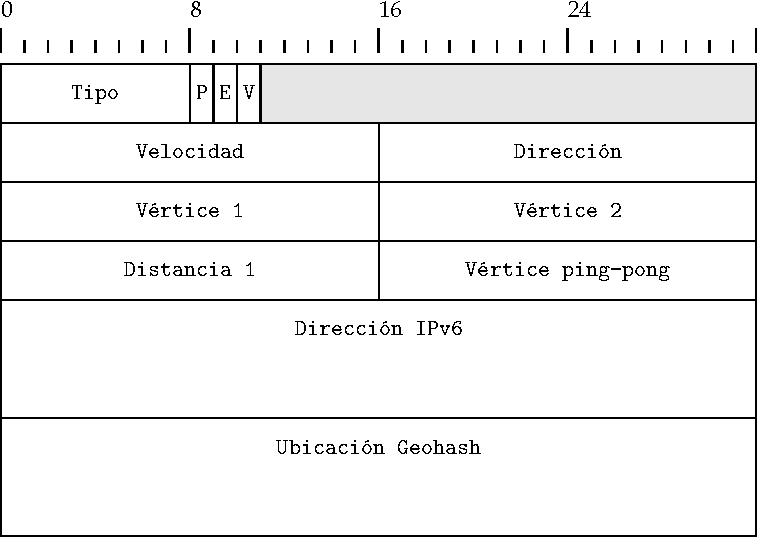
\includegraphics{formato_anc_vehic}
\decoRule
\caption[Formato del mensaje ANC-VEHIC]{Formato del mensaje ANC-VEHIC.}
\label{fig:formato_anc_vehic}
\end{figure}

\keyword{Tipo (8 bits)} -- Su valor es \code{1} para indicar que se trata de un
mensaje ANC-VEHIC.

\keyword{P (1 bit)} -- Si vale 1, indica si el mensaje anuncia el resultado de
una operación ping-pong.

\keyword{E (1 bit)} -- Si vale 1, indica que hubo un error en la operación
ping-pong, lo que significa que la arista que se anuncia está inactiva.
Únicamente es válido si la bandera \keyword{P} vale 1.

\keyword{Dirección (16 bits)} -- Ángulo acimutal de la dirección del movimiento
del vehículo en grados.

\keyword{Velocidad (16 bits)} -- Velocidad del vehículo en m/s.

\keyword{Vértice A (16 bits)} -- Primer vértice de la arista por la que
circula el vehículo.

\keyword{Vértice B (16 bits)} -- Segundo vértice de la arista por la que
circula el vehículo.

\keyword{Distancia A (16 bits)} -- Distancia en metros del vehículo al vértice
A.

\keyword{Vértice ping} -- Vértice de origen de la operación ping-pong.
Únicamente es válido si la bandera \keyword{P} vale 1.

\keyword{Vértice pong} -- Vértice de destino de la operación ping-pong.
Únicamente es válido si la bandera \keyword{P} vale 1.

\keyword{Dirección IPv6 (128 bits)} -- Dirección IPv6 del vehículo que
transmite el mensaje.

\keyword{Ubicación Geohash (64 bits)} -- Ubicación Geohash de longitud 12 del
vehículo al momento de transmitir el mensaje.

%-----------------------------------
%   MENSAJE ANUNCIO-HOST
%-----------------------------------
\subsection{Anuncio-\textit{host} (ANC-HOST)}

\label{subsec:mensaje_anuncio_host}

El mensaje ANC-HOST tiene una longitud de 28 octetos, y su formato se muestra
en la figura \ref{fig:formato_anc_host}. Los campos del mensaje son los
siguientes:

\begin{figure}[th!]
\centering
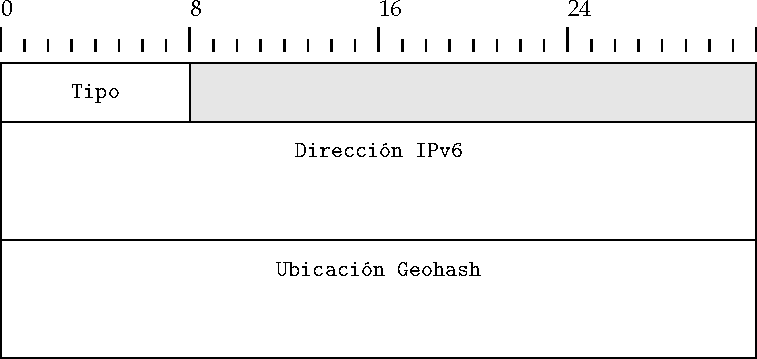
\includegraphics{formato_anc_host}
\decoRule
\caption[Formato del mensaje ANC-HOST]{Formato del mensaje ANC-HOST.}
\label{fig:formato_anc_host}
\end{figure}

\keyword{Tipo (8 bits)} -- Su valor es \code{2} para indicar que se trata de un
mensaje ANC-HOST.

\keyword{Dirección IPv6 (128 bits)} -- Dirección del \textit{host} que emite el
mensaje.

\keyword{Ubicación Geohash (65 bits)} -- Ubicación Geohash del \textit{host} al
momento de transmitir el mensaje.

%-----------------------------------
%   MENSAJE PING
%-----------------------------------
\subsection{Ping (PING)}

\label{subsec:mensaje_ping}

El mensaje PING tiene una longitud de 24 octetos, y su formato se muestra en la
figura \ref{fig:formato_ping}. Los campos del mensaje son los siguientes:

\begin{figure}[th!]
\centering
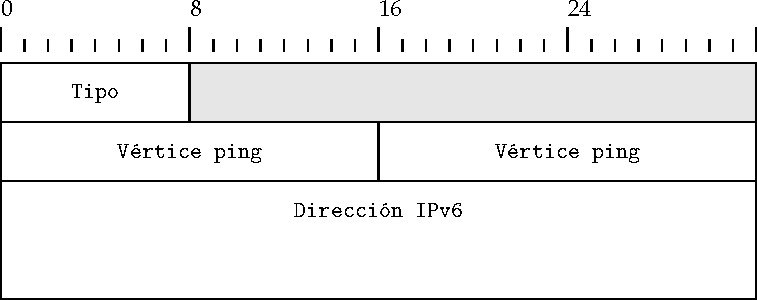
\includegraphics{formato_ping}
\decoRule
\caption[Formato del mensaje PING]{Formato del mensaje PING.}
\label{fig:formato_ping}
\end{figure}

\keyword{Tipo (8 bits)} -- Su valor es \code{3} para indicar que se trata de un
mensaje PING.

\keyword{Vértice ping (16 bits)} -- Vértice de origen de la operación
ping-pong.

\keyword{Vértice ping (16 bits)} -- Vértice de destino de la operación
ping-pong.

\keyword{Dirección IPv6 (128 bits)} -- Dirección IPv6 del vehículo que originó
el mensaje.

%-----------------------------------
%   MENSAJE PONG
%-----------------------------------
\subsection{Pong (PONG)}

\label{subsec:mensaje_pong}

El mensaje PONG tiene una longitud de 24 octetos, y su formato se muestra en la
figura \ref{fig:formato_pong}. Los campos del mensaje son los siguientes:

\begin{figure}[th!]
\centering
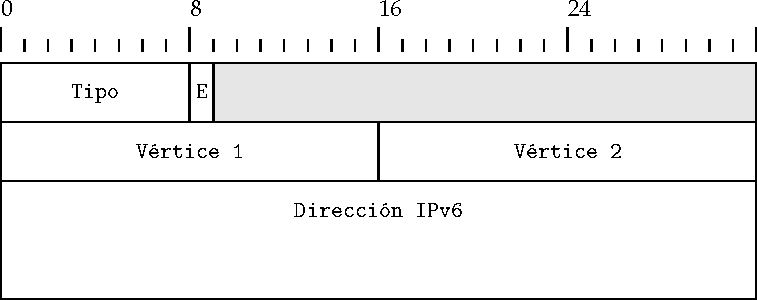
\includegraphics{formato_pong}
\decoRule
\caption[Formato del mensaje PONG]{Formato del mensaje PONG.}
\label{fig:formato_pong}
\end{figure}

\keyword{Tipo (8 bits)} -- Su valor es \code{4} para indicar que se trata de un
mensaje PONG.

\keyword{E (1 bit)} -- Si vale \code{1}, indica que hubo un error en la
operación ping-pong.

\keyword{Vértice ping (16 bits)} -- Vértice de origen de la operación
ping-pong.

\keyword{Vértice pong (16 bits)} -- Vértice de destino de la operación
ping-pong.

\keyword{Dirección IPv6 (128 bits)} -- Dirección del vehículo que originó el
mensaje PING que responde.

%-----------------------------------
%   DIRECTORIO DE VEHÍCULOS VECINOS
%-----------------------------------
\section{Directorio de vehículos vecinos}

\label{sec:directiorio_vehiculos_vecinos}

\begin{sloppypar}
Los vehículos informan sobre su disponibilidad por medio de mensajes
\mbox{ANC-VEHIC}, en los que se incluye información sobre su ubicación vial. La
frecuencia con la que los vehículos transmiten estos mensajes se determina con
el parámetro \mbox{INTERVALO\_ANC\_VEHIC}. Para que todos los vehículos puedan
recibir estos mensaje, éste se dirige a la dirección \textit{multicast} de la
subred.
\end{sloppypar}

Cada vehículo tiene un \keyword{directorio de vehículos vecinos}, que le
permite mantener un registro de los vehículos que se encuentran cerca. Esta
información le ayuda a determinar el siguiente salto al enrutar un paquete.
Cada registro en el directorio de vehículos vecinos contiene los siguientes
campos:

\begin{center}
\begin{tabular}{ r l }
Dirección IP: & Tiempo de expiración \\
& Ubicación \\
& Velocidad \\
& Dirección de movimiento \\
& Vértice A \\
& Vértice B \\
& Distancia a A \\
& Distancia a B
\end{tabular}
\end{center}

Cada registro se identifica con la dirección IP del vehículo, y los campos de
cada registro son los siguientes:

\keyword{Tiempo de exporación} -- Tiempo hasta el que el registro es válido.

\keyword{Ubicación Geohash} -- Ubicación del vehículo.

\keyword{Velocidad} -- Velocidad del vehículo en m/s.

\keyword{Dirección del movimiento} -- Ángulo acimutal de la dirección del
movimiento del vehículo en grados.

\keyword{Vértice A} -- Primer vértice de la arista por la que
circula el vehículo. Es el vértice hacia el que se dirige el vehículo.

\keyword{Vértice B} -- Segundo vértice de la arista por la que
circula el vehículo.

\keyword{Distancia A} -- Distancia al vértice A.

\keyword{Distancia B} -- Distancia al vértice B.

\begin{sloppypar}
Cuando un vehículo recibe un mensaje ANC-VEHIC, obtiene la ubicación vial del
vecino. Si no hay un registro con la dirección IP, se crea uno nuevo, y si ya
existe, se actualiza el registro. El tiempo de expiración se obtiene a partir
del valor del parámetro VIGENCIA\_VEHICULO\_VECINO, y se actualiza cada vez que
llega un mensaje del vehículo correspondiente.
\end{sloppypar}

Si un vehículo deja de recibir mensajes ANC-VEHIC de otro, el tiempo de
expiración del registro deja de actualizarse, y cuando se cumple este tiempo,
se asume que el enlace hacia tal vehículo se terminó y se elimina el registro.

%-----------------------------------
%   DIRECTORIO DE HOSTS VECINOS
%-----------------------------------
\section{Directorio de \textit{hosts} vecinos}

\label{sec:directorio_hosts_vecinos}

De manera similar, los \textit{hosts} que necesiten comunicarse a través de
la VANET se anuncian ante los vehículos vecinos. Esto lo hacen enviando su
dirección IP y su ubicación en mensajes ANC-HOST a la dirección
\textit{multicast}. La frecuencia con la que un \textit{host} transmite estos
mensajes se especifica con el parámetro INTERVALO\_ANC\_HOST

Únicamente los vehículos pueden procesar los mensajes ANC-HOST, y tienen un
\keyword{directorio de hosts vecinos}, donde registran los \textit{hosts} de
los que han recibido algún mensaje ANC-VEHIC recientemente. Cada registro
contiene los siguientes datos:

\begin{center}
\begin{tabular}{ r l }
Dirección IP: & Tiempo de expiración \\
& Ubicación \\
\end{tabular}
\end{center}

Los campos de cada registro del directorio son los siguientes:

\keyword{Tiempo de exporación} -- Tiempo hasta el que el registro es válido.

\keyword{Ubicación} -- Ubicación del \textit{host}.

Al igual que en el directorio de vehículos vecinos, cada registro tiene un
tiempo de validez, que se define con el parámetro VIGENCIA\_HOST\_VECINO, y se
actualiza cada vez que se recibe un mensaje ANC-HOST. Si se cumple el tiempo de
expiración de un registro, este se elimina.

%-----------------------------------
%   PING-PONG
%-----------------------------------
\section{Operación ping-pong}

\label{sec:operacion_ping_pong}

Tener una ruta vial no significa que existan vehículos en todas la aristas a
lo largo de la ruta. Por lo tanto, es importante verificar si en una arista hay
vehículos que puedan retransmitir un paquete para que llegue al otro extremo de
esta. La operación ping-pong sirve para verificar si se cumple esta condición
en una arista.

Una operación ping-pong comienza cuando un vehículo que se encuentra en un
vértice origina un mensaje PING, el cual retransmite hacia algún vehículo
vecino que se encuentra en la arista de interés, si es que hay. En este
mensaje, el campo \keyword{vértice 1} indica el vértice donde se inicia la
operación, y el vértice al que debe llegar se indica en el campo
\keyword{vértice 2}. El mensaje también lleva la dirección IP del vehículo que
lo originó. La figura \ref{fig:recorrido_ping} muestra el recorrido de un
mensaje PING para llegar de un vértice al otro.

\begin{figure}[th!]
\centering
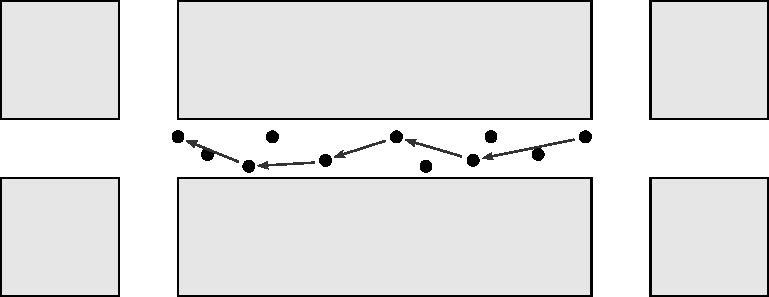
\includegraphics{recorrido_ping}
\decoRule
\caption[Recorrido de un mensaje PING]{Recorrido de un mensaje PING.}
\label{fig:recorrido_ping}
\end{figure}

El mensaje PING se retransmite entre los vehículos hasta llegar a alguno que se
encuentre en el otro vértice de la arista. Este vehículo responde con un
mensaje PONG, que se retransmite de regreso hasta llegar al vehículo que inició
la operación. En este mensaje, la bandera \keyword{E} tiene un valor de 0, para
indicar que el mensaje PING llegó al vértice. El campo \keyword{vértice 1}
indica el vértice donde se originó el mensaje PING, y el campo \keyword{vértice
2} indica el vértice al que tenía que llegar. En la figura
\ref{fig:recorrido_pong} se muestra el recorrido de un mensaje PONG para llegar
al vehículo que inició la operación.

\begin{figure}[th!]
\centering
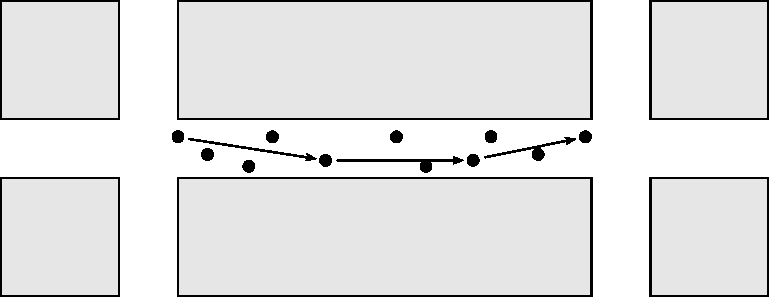
\includegraphics{recorrido_pong}
\decoRule
\caption[Recorrido de un mensaje PONG]{Recorrido de un mensaje PONG.}
\label{fig:recorrido_pong}
\end{figure}

Si un vehículo recibe un mensaje PING pero no encuentra un vecino al que
retransmitirlo, éste responde con un mensaje PONG, asignando el valor 1 a la
bandera \keyword{E} para indicar que no se completó la operación, lo que
significa que el vértice de destino no se puede alcanzar.

Cuando un vehículo que inició la operación recibe el mensaje PONG de respuesta,
y la bandera de error \keyword{E} tiene un valor de 0, se dice que la arista es
una \keyword{arista activa}. En este caso, el vehículo transmite un mensaje
ANC-VEHIC, en el que la bandera \keyword{P} tiene el valor 1 para anunciar el
resultado de una operación ping-pong, el vértice de destino de la operación se
indica en el campo \keyword{vértice ping-pong}, y la bandera \keyword{E} tiene
valor de 0 para decir que la arista está activa. Este mensaje también incluye
la ubicación vial del vehículo, igual que los mensajes ANC-VEHIC que se
transmiten periódicamente.

El vehículo que inicia una operación ping-pong establece un tiempo de espera,
definido por el parámetro ESPERA\_PONG. Si el tiempo de espera se agota, o si
recibe un mensaje PONG de respuesta con el valor 1 en la bandera de error
\keyword{E}, se transmite un mensaje ANC-VEHIC, pero con la bandera \keyword{E}
con el mismo valor para anunciar que la arista está inactiva.

Cuando el mensaje PING logra atravesar la arista y llega a un vehículo en el
vértice deseado, después de responder con el mensaje PONG, este vehículo
también anuncia, con un mensaje ANC-VEHIC, que la arista está activa.

%-----------------------------------
%   ARISTAS ACTIVAS E INACTIVAS
%-----------------------------------
\subsection{Aristas activas e inactivas}

\label{subsec:aristas_activas_e_inactivas}

Con la operación ping-pong es posible saber si hay vehículos que puedan
retransmitir paquetes de un vértice a otro. Esto es importante a la hora del
cálculo de las rutas viales, por lo que cada vehículo tiene un registro de
aristas activas y otro de aristas inactivas.

Cuando se recibe un mensaje ANC-VEHIC que indica el resultado de una operación
ping-pong, se revisa el campo \keyword{vértice ping-pong} y la bandera
\keyword{V} para saber de qué arista se trata, y se agrega al \keyword{registro
de aristas activas}, junto con su tiempo de validez determinado por el
parámetro VIGENCIA\_ARISTA\_ACTIVA. Si la arista ya está registrada, se
actualiza el tiempo de validez. Se asume que la arista está activa hasta que
se agota el tiempo de validez. Una vez que se agota, se elimina del registro y
se desconoce el estado de la arista, hasta la siguiente actualización.

Si se recibe un mensaje ANC-VEHIC una arista inactiva, se revisa para saber de
qué arista se trata, y se agrega al \keyword{registro de aristas inactivas}
junto con un tiempo de validez definido por el parámetro
VIGENCIA\_ARISTA\_INACTIVA. Si ya la arista vértice ya existe en el registro,
se actualiza el tiempo de validez. Si este tiempo se agota, se elimina del
registro.

%-----------------------------------
%   ENRUTAMIENTO
%-----------------------------------
\section{Enrutamiento}

\label{sec:enrutamiento}

En las siguientes secciones, se presenta el proceso que lleva a cabo un vehículo
cuando recibe un paquete para enrutar.

%-----------------------------------
%   CÓMPUTO DE RUTAS VIALES
%-----------------------------------
\subsection{Cómputo de rutas viales}

\label{subsec:computo_rutas_viales}

Para tratar de evitar pérdida de paquetes por obstrucciones de edificios, se
busca que las rutas incluyan la menor cantidad de giros en esquinas posible.
En la figura \ref{fig:ruta_mala} se muestra una ruta del vértice $d$ al vértice
$i$ en la que hay giros en cuatro esquinas. Si un paquete siguiera esa ruta, en
cada uno de los giros habría posibilidad de chocar con el edificio de la
esquina.

\begin{figure}[th!]
\centering
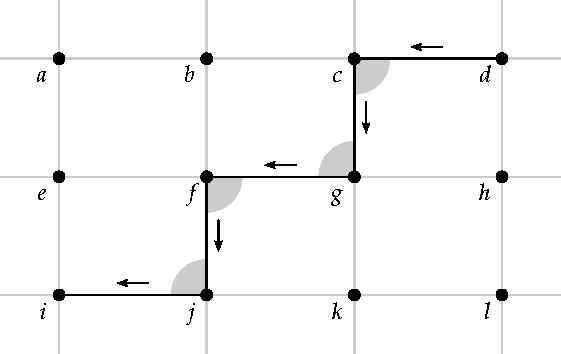
\includegraphics{ruta_mala}
\decoRule
\caption[Ruta con muchos giros en esquinas]{Ruta con muchos giros en
esquinas.}
\label{fig:ruta_mala}
\end{figure}

En cambio, en la figura \ref{fig:ruta_buena} se muestra otra ruta que une los
mismos vértices, pero esta únicamente incluye un giro. Si un paquete siguiera
esta ruta, sólo correría el riesgo de chocar con algún edificio en un giro. Por
esta razón, la busqueda de rutas viales debe considerar tramos rectos lo más
largos que sea posible.

\begin{figure}[th!]
\centering
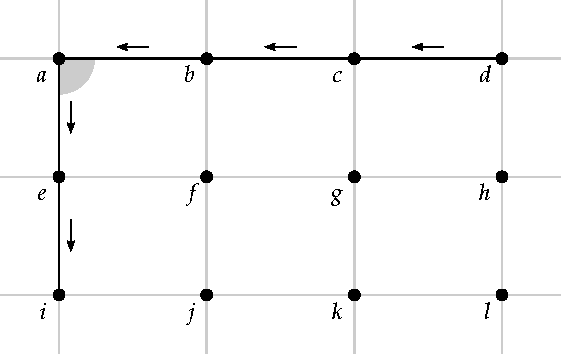
\includegraphics{ruta_buena}
\decoRule
\caption[Ruta con un giro en una esquinas]{Ruta con un giro en una
esquinas.}
\label{fig:ruta_buena}
\end{figure}

Para utilizar un algoritmo para determinar las rutas en el grafo vial, es
necesario asignar un peso a cada una de las aristas. Sin embargo, para generar
rutas con el criterio descrito anteriormente, el peso de cada arista depende de
la arista anterior. Por ejemplo, en la ruta de la figura \ref{fig:ruta_mala},
para ir de la arista $\{d,c\}$ a la arista $\{c,g\}$, hay un giro de ángulo
considerable, mientras que en la ruta de la figura \ref{fig:ruta_buena}, para
ir de la arista $\{d,c\}$ a la arista $\{c,b\}$, el tramo es recto, por lo que
la arista $c,b\}$ tendrá un peso menor que la arista $d,g\}$ respecto a la
arista $\{d,c\}$.

Existen algoritmos para grafos que calculan la ruta más corta desde un vértice
inicial al resto de los vértices, como el algoritmo de Dijkstra
\cite{cormen2001}. Sin embargo, este algoritmo asume que las aristas tienen un
peso fijo previamente asignado. Por este motivo, se propone un algoritmo
inspirado en el algoritmo de Dijkstra, pero que hace la búsqueda de las rutas a
partir de los dos vértices de una arista inicial. Además, el peso de cada
arista se calcula conforme el algoritmo progresa, y descarta un conjunto de
aristas inactivas y los vértices por los que el paquete ya ha pasado.

En la figura \ref{fig:angulos_aristas}, la flecha indica la dirección de la
arista $\{a,b\}$, y se muestran los ángulos que forma esta con la dirección de
cada una de las demás aristas. Estos ángulos van a funcionar como el peso de su
respectiva arista. Debido a que $\{b,d\}$ forma el menor ángulo con la
dirección de $\{a,b\}$, ésta tiene el menor peso, y $\{b,c\}$ tendrá el mayor
peso, ya que su ángulo es el mayor. De este modo, la ruta contendrá la menor
cantidad de giros pronunciados en los cruces viales.

\begin{figure}[th!]
\centering
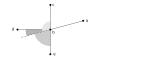
\includegraphics{angulos_aristas}
\decoRule
\caption[Determinación del peso de las aristas con sus ángulos de
dirección]{Determinación del peso de las aristas con sus ángulos de dirección.}
\label{fig:angulos_aristas}
\end{figure}

\begin{algorithm}[th!]
\small
\caption{Cálculo de la ruta más corta}
\label{alg:ruta_mas_corta}
\DontPrintSemicolon
\LinesNumbered
    \KwData{$\{a,b\}$: Arista inicial, $\mathbf{G}$: Grafo vial, $VV$: Conjunto
    de vértices visitados, $AE$: Conjunto de aristas activas}
    \Begin{
        \ForEach{$v \in \mathbf{G}.\mathbf{V}$} {
            $distancias[v] \gets \infty$ \;
        }
        $distancias[a] \gets 0$ \;
        $distancias[b] \gets 0$ \;
        $S \gets \mathbf{G.V} \setminus \{a,b\}$ \;
        \ForEach{$v \in \mathbf{G}.\mathbf{V}$ adyacente a $a$}{
            \If{$v \neq b$}{
                \eIf{$v \notin VV$ y $\{a,v\} \in AE$}{
                    $distancias[v] \gets calcularPeso(\{a,v\}, \{a,b\})$ \;
                    $predecesores[v] \gets a$ \;
                }{
                    $S \gets S \setminus \{v\}$ \;
                }
            }
        }
        \ForEach{$v \in \mathbf{G}.\mathbf{V}$ adyacente a $b$}{
            \If{$v \neq a$}{
                \eIf{$v \notin VV$ y $\{b,v\} \in AE$}{
                    $peso \gets calcularPeso(\{b,v\}, \{a,b\}$) \;
                    \If{$peso < distancias[v]$}{
                        $distancias[v] \gets peso$ \;
                        $predecesores[v] \gets b$ \;
                    }
                }{
                    $S \gets S \setminus \{v\}$ \;
                }
            }
        }
        \While{$S \neq \emptyset$}{
            $v \gets$ vértice en $S$ con menor distancia \;
            $u \gets predecesores[v]$ \;
            \ForEach{$w \in \mathbf{G}.\mathbf{V}$ adyacente a $v$}{
                \If{$w \neq u$}{
                    \eIf{$w \notin VV$}{
                        $peso \gets calcularPeso(\{v,w\}, \{u,v\})$ \;
                        \If{$distancias[w] > distancias[v] + peso$}{
                            $distancias[w] \gets distancias[v] + peso$ \;
                            $predecesores[w] \gets v$ \;
                        }
                    }{
                        $S \gets S \setminus \{w\}$ \;
                    }
                }
            }
            $S \gets S \setminus \{v\}$ \;
        }
        \Return{predecesores, distancias}
    }
\end{algorithm}

El algoritmo \ref{alg:ruta_mas_corta} es el algoritmo propuesto, donde se
definen dos vectores cuyo tamaño es igual al número de vértices en el grafo. El
vector $predecesores$ indica cuál es el vértice predecesor de cada uno en la
ruta. El vector $distancias$ indica la distancia desde la arista de inicia
hacia cada vértice. En este contexto, se entiende como distancia a la suma de
los pesos de todas las aristas que forman una ruta, por lo que se denomina
\keyword{distancia de ruta}, para evitar confusión. También se define un
conjunto llamado $S$, que contiene los vértices cuya ruta falta obtener.

El algoritmo recibe la arista inicial $\{a,b\}$, el grafo vial $\mathbf{G}$,
el conjunto de vértices no disponibles $NV$ y el conjunto de aristas inactivas
$NE$. En las líneas 3-6, se establece la distancia de ruta a cada vértice como
$\infty$, excepto para los vértices iniciales, cuya distancia de ruta es 0. En
la línea 7 se agregan todos los vértices a $S$, excepto los dos iniciales.

En las líneas 8-12, se calcula y actualiza la distancia de ruta a los vértices
adyacentes a $a$, excepto los vétices no disponibles. En las líneas 13-19, se
hace el mismo procedimiento, pero para los vértices adyacentes a $b$, y después
se procede a procesar el resto de los vértices. Debido a que la distancia de
ruta de los vértices no disponibles nunca deja de ser $\infty$, en la línea 21
se verifica si existe un vértice $u$ en $S$ cuya distancia de ruta ya se haya
calculado anteriormente, es decir, que se puede alcanzar mediante un vértice ya
procesado. Si no hay, se termina el algoritmo, pero si sí hay, se calcula la
distancia de ruta hacia cada uno de sus vértices adyacentes, y se actualiza si
es una distancia de ruta menor a la que ya tenía, en cuyo caso, se asigna $u$
como su predecesor.

El resultado final son los vectores $predecesores$ y $distancias$. Con el
vector $predecesores$, para determinar la ruta hacia un vértice $u$, se busca
su predecesor $v$. Después, se busca $v$ y se obtiene su predecesor $w$, y esto
se repite hasta llegar a alguno de los dos vértices iniciales. Con el vector
$distancias$ se puede saber si se encontró alguna ruta hacia cierto vértice. Si
su distancia de ruta es $\infty$, significa que no se encontró.

%-----------------------------------
%   VERIFICACIÓN DE LA CABECERA DE OPCIONES DE SALTO POR SALTO
%-----------------------------------
\subsection{Verificación de la cabecera de opciones de salto por salto}

\label{subsec:verificacion_cabecera_opciones_salto_por_salto}

Cuando un vehículo recibe un paquete, primero debe verificar si este contiene
la cabecera de opciones de salto por salto. De ser así, verifica si esta
cabecera tiene la opción de ubicación del destino. Si no la tiene, se descarta
el paquete, ya que no hay manera de saber hacia dónde tiene que llegar.
Después, se verifica si el destino del paquete se encuentra en la misma subred,
en cuyo caso, se revisa si la cabecera tiene la opción de ubicación vial del
destino. Si no la tiene, esta se calcula y se agrega a la cabecera. Del mismo
modo, se verifica si la cabecera tiene la opción de vértices visitados, y si no
es así, se agrega. El algoritmo \ref{alg:validar_cabeceras_paquete} muestra
este procedimiento de validación de la cabecera de los paquetes.

\begin{algorithm}[th!]
\small
\caption{Validar cabecera de opciones de salto por salto de paquete}
\label{alg:validar_cabeceras_paquete}
\DontPrintSemicolon
\LinesNumbered
    \KwData{$paquete$: Paquete a enrutar}
    \Begin{
        \If{$paquete$ no contiene cabecera de opciones de salto por salto}{
            \Return{$Falso$}
        }
        $cabecera \gets$ cabecera de opciones de salto por salto de $paquete$ \;
        \If{$cabecera$ no contiene opción de ubiación de destino}{
            \Return{$Falso$}
        }
        $ubicVehic \gets$ ubicación del vehículo \;
        $ubicDest \gets$ ubicación del \textit{host} destino en $cabecera$ \;
        \If{$ubicVehic$ y $ubicDest$ están en la misma región Geohash }{
            \If{$cabecera$ no contiene opción de ubicación vial de destino}{
                $ubicVialDest \gets CalcularUbicacionVial(ubicDest)$ \;
                agregar $ubicVialDest$ a $cabecera$ \;
           }
        }
        \If{$cabecera$ no contiene opción de vértices visitados}{
            agregar opción de vértices visitados vacía a $cabecera$ \;
        }
        \Return{$Verdadero$}
    }
\end{algorithm}

%-----------------------------------
%   VÉRTICE DESTINO LOCAL
%-----------------------------------
\subsection{Vértice destino local}

\label{subsec:vertice_destino_local}

Después de revisar la cabecera, se debe seleccionar el \keyword{vértice destino
local} dentro de la subred. Se dice que es local porque es el último vértice,
\keyword{dentro de la red vial local}, al que el paquete debe llegar para
seguir su camino hacia al \textit{host} destino. Si el \textit{host} destino
está en la misma subred, el vértice destino local será uno de los dos vértices
de la ubicación vial de este. Si el \textit{host} destino se encuentra en otra
subred, el vértice destino local será un vértice \textit{gateway} que le
permita llegar a la siguiente subred en la ruta interregión enrutamiento.

El algoritmo \ref{alg:vertice_destino_local} describe cómo se determina el
vértice destino local. Primero, se calcula la ruta más corta con el algoritmo
\ref{alg:ruta_mas_corta} desde la ubicación vial del vehículo al resto de los
vértices (línea 8). Si el \textit{host} destino está en la misma subred, se
obtienen los dos vértices de su ubicación vial, y el vértice destino local será
el que tenga una menor distancia de ruta (líneas 11-17).

Si el \textit{host} destino está en otra subred, se lleva a cabo un
enrutamiento interregión. Esto sifgnifica que el paquete debe pasar a otra
subred que lo acerque a la subred de destino. Para esto, se debe conocer en qué
dirección se encuentra la subred de destino respecto a la subred local, tanto
en latitud como en longitud. Las subredes vecinas que se encuentran a cada
dirección se denominan \keyword{siguientes subredes tentativas}, ya que aún no
se conoce cuál será la siguiente subred en la ruta interregión. Se define el
conjunto $verticesGateway$, que va a contener los vértices a través de los
cuales el vértice puede llegar a alguna de las siguientes subredes tentativas.
Si la subred destino se encuentra al norte, se agregan al conjunto
$verticesGateway$ los vértices \textit{gateway} al norte del grafo vial local
(líneas 22-23). Si se encuentra al sur, se agregan los vértices
\textit{gateway} al sur del grafo vial local (líneas 24-26). Por otro lado, si
la subred destino se encuentra al este, se agregan los vértices
\textit{gateway} al este (líneas 27-28), y si se encuentra al oeste, se agregan
los vértices \textit{gateway} al oeste (líneas 29-31). Finalmente, se busca en
$verticesGateway$ el vértice cuya distancia de ruta sea la menor, y ese se
seleciona como vértice destino local (línea 32).

\begin{figure}[th!]
\centering
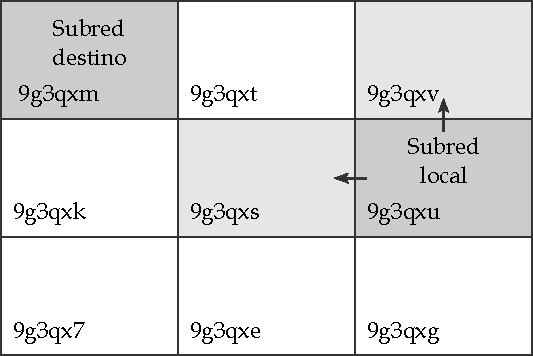
\includegraphics{siguiente_subred_tentativa}
\decoRule
\caption[Siguientes subredes tentativas]{Siguientes subredes tentativas.}
\label{fig:siguiente_subred_tentativa}
\end{figure}

\begin{algorithm}[th!]
\small
\caption{Obtener vétice de destino local}
\label{alg:vertice_destino_local}
\DontPrintSemicolon
\LinesNumbered
    \KwData{$paquete$: Paquete a enrutar}
    \Begin{
        $cabecera \gets$ cabecera de opciones de salto por salto de $paquete$ \;
        $ubicVialVehic \gets$ ubicación vial del vehículo \;
        $NV \gets$ vértices visitados en $cabecera$ \;
        $NE \gets$ aristas inactivas \;
        $\mathbf{G} \gets$ grafo vial de la subred \;
        $pred, dist \gets
            RutaMasCorta(ubicVialVehic.arista, \mathbf{G}, NV, NE)$ \;
        $ubicVehic \gets$ ubicación del vehículo \;
        $ubicDest \gets$ ubicación del \textit{host} destino en $cabecera$ \;
        \eIf{$ubicVehic$ y $ubicHost$ están en la misma región Geohash}{
            $ubicVialHost \gets$ ubicación vial del \textit{host} destino en
            $cabecera$ \;
            $\{a,b\} \gets ubicVialHost.arista$ \;
            \eIf{$dist[a] < dist[b]$}{
                $verticeDestino \gets a$ \;
            }{
                $verticeDestino \gets b$ \; 
                
            }
        }{
            $regionLocal \gets$ región Geohash local \;
            $regionDest \gets$ región Geohash de destino \;
            $verticesGateway \gets \emptyset$ \;
            \eIf{$regionDest$ está al norte de $regionLocal$}{
                $verticesGateway \gets verticesGateway \cup$ vértices
                    \textit{gateway} en $\mathbf{G}$ al norte \;
            }{
                \If{$regionDest$ está al sur de $regionLocal$}{
                    $verticesGateway \gets verticesGateway \cup$ vértices
                        \textit{gateway} en $\mathbf{G}$ al sur \;
                }
            }
            \eIf{$regionDest$ está al este de $regionLocal$}{
                $verticesGateway \gets verticesGateway \cup$ vértices
                    \textit{gateway} en $\mathbf{G}$ al este \;
            }{
                \If{$regionDest$ está al oeste de $regionLocal$}{
                $verticesGateway \gets verticesGateway \cup$ vértices
                    \textit{gateway} en $\mathbf{G}$ al oeste \;
                }
            }
            $verticeDestino \gets$ vértice en $verticesGateway$ cuya distancia
                de ruta en $dist$ sea la menor \; }
        \Return{$verticeDestino$}
    }
\end{algorithm}

En la figura \ref{fig:siguiente_subred_tentativa}, hay un paquete en la subred
9g3qxu cuyo destino está en la subred 9g3qxm. La subred destino se encuentra al
noroeste de la subred local, por lo que hay dos \keyword{siguientes subredes
tentativas}, la que se encuentra al norte y la que se encuentra al oeste, que
son 9g3qxv y 9g3qxs, respectivamente. Para determinar cuál de estas dos será la
siguiente subred, primero se obtienen los vértices \textit{gateway} de la red
vial local que llevan a estas dos subredes, es decir, los del norte y los del
oeste. Después, se selecciona el vértice cuya distancia de ruta sea la menor, y
este será el vértice de destino local.

%-----------------------------------
%   SELECCIÓN DEL SIGUIENTE SALTO
%-----------------------------------
\subsection{Selección del siguiente salto}

\label{subsec:seleccion_siguiente_salto}

Una vez que se conoce el vértice destino local, se debe seleccionar un vehículo
vecino para retransmtir el paquete. Se busca que el paquete haga el mayor
avance posible con cada retransmisión, por lo que se debe seleccionar un vecino
que se encuentre lejos, pero con el que se tenga línea de visión. Las
distancias de ruta de cada vértice ayudan a determinar con qué vecinos es
probable que haya línea de visión. En la figura
\ref{fig:ruta_siguiente_salto_1}, el vehículo $V_1$ circula por la arista
$\{h,g\}$, y debe enrutar un paquete cuyo último vértice de destino es $i$.
Después de calcular la ruta más corta, obtiene la ruta $h \rightarrow g
\rightarrow f \rightarrow e \rightarrow i$. Como $g$ y $h$ son los vértices de
la arista inicial en la ruta, su distancia de ruta es 0, como se explicó en la
sección \ref{subsec:computo_rutas_viales}. El ángulo que forma la arista
$\{g,f\}$ con la dirección de la arista $\{h,g\}$ es 0\si{\degree}, por lo que su
peso $f$ será 0. El ángulo que forma la arista $\{f,e\}$ con la arista
$\{g,f\}$ también es 0, por lo que su peso también es 0. El peso de la arista
$\{e,i\}$ es 90, ya que esta forma un ángulo de 90\si{\degree} con la arista
anterior. Con estos pesos, la distancia de ruta de los vértices $f$, $e$ e $i$
son 0, 0 y 90, respectivamente. Con lo que se puede deducir que $e$ es el
último vértice con el que es probale tener una línea de visión desde la arista
inicial.

\begin{figure}[th!]
\centering
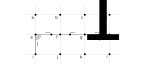
\includegraphics{ruta_siguiente_salto_1}
\decoRule
\caption[Ruta con secuencia de varias aristas con línea de visión]{Ruta con
secuencia de varias de aristas con línea de visión.}
\label{fig:ruta_siguiente_salto_1}
\end{figure}

En la figura \ref{fig:ruta_siguiente_salto_2} se muestra la misma ruta, pero
con los vehículos $V_2$ y $V_3$ circulando en las arista $\{g,f\}$, y $V_4$ en
$\{f,e\}$. Se indica que la arista $\{f,g\}$está activa para $V_1$,
pero no la arista $\{f,e\}$. Por esta razón, a pesar de que $V_1$ tiene línea
de visión con $e$, se descartan como siguiente salto los vehículos circulando
por $\{f,e\}$. El último vértice alcanzable en la ruta, y con el que se tiene
línea de visión, es $f$, por lo que sí se consideran los vehículos circulando
en $\{g,f\}$ para seleccinar el siguiente salto. Los vehículos vecinos que
circulan en esa arista son $V_2$ y $V_3$, pero para que el paquete avance lo
más posible, se selecciona como siguiente salto el más cercano a $f$, que es
$V_3$.
% Una vez seleccionado el siguiente salto, $V_1$ agrega una ruta nueva a
% su tabla de enrutamiento, en la que el destino es la dirección IP de destino
% del paquete, y el siguiente salto la dirección IP de $V_2$. Además, se
% establece un tiempo de validez de la ruta, definido por el parámetro
% VIGENCIA\_RUTA.

\begin{figure}[th!]
\centering
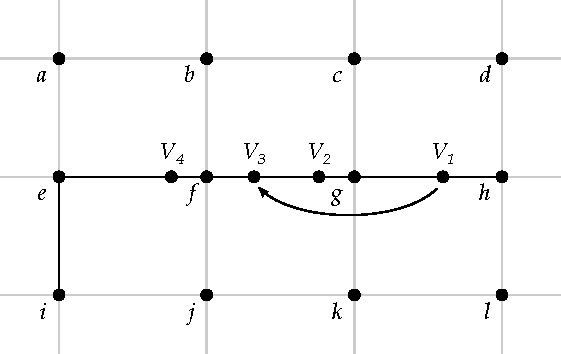
\includegraphics{ruta_siguiente_salto_2}
\decoRule
\caption[Selección del siguiente salto en ruta con secuencia de varias de
aristas con línea de visión]{Selección del siguiente salto en ruta con
secuencia de varias de aristas con línea de visión.}
\label{fig:ruta_siguiente_salto_2}
\end{figure}

Otra ruta se muestra en la figura \ref{fig:ruta_siguiente_salto_3}, la cual
inicia en la arista $\{d,c\}$, donde circula el vehículo $V_1$ y tiene como
destino el vértice $k$. En este caso, el siguiente vértice en la ruta es $g$, y
tiene una distancia de ruta de 90, debido a que el ángulo que forma la arista
$\{c,g\}$ con la dirección de la arista $\{d,c\}$ es de 90\si{\degree}. En esta ruta, la
única arista donde $V_1$ tiene línea de visión es la arista inicial $\{d,c\}$,
por lo que únicamente podría transitir los paquetes a vehículos vecinos en la
misma arista.

\begin{figure}[th!]
\centering
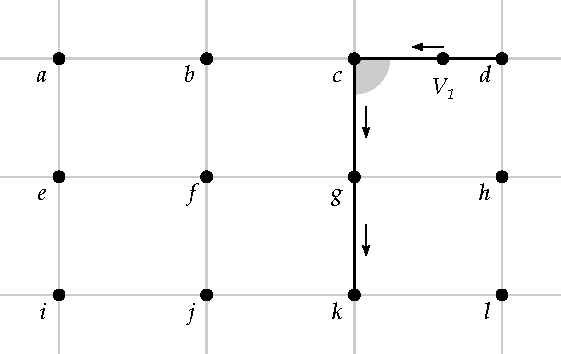
\includegraphics{ruta_siguiente_salto_3}
\decoRule
\caption[Ruta sin secuencia de varias aristas con línea de visión]{Ruta sin
secuencia de varias aristas con línea de visión.}
\label{fig:ruta_siguiente_salto_3}
\end{figure}

En la figura \ref{fig:ruta_siguiente_salto_4}, se muestra la misma ruta, además
de los vehículos $V_1$ y $V_2$ circulando en la arista $\{d,c\}$, $V_3$
circulando en $\{c,g\}$, y $V_4$ circulando en $\{g,k\}$. El vehículo $V_1$
tiene un paquete que tiene que seguir la ruta, pero este sólo tiene línea de
visión con los vehículos en la arista $\{d,c\}$. En este escenario, el último
vértice alcanzable con línea de visión en la ruta es $c$, por lo que $V_1$ debe
seleccionar como siguiente salto un vehículo que acerque el paquete  a este
vértices; en este caso, se trata de $V_2$. El vértice $V_2$ se encuentra en el
vértice $c$, y, desde su ubicación, el último vértice alcanzable con línea de
visión es $k$. Por este motivo, busca el vehículo vecino más cercano al vértice
$k$, que en este caso es $V_4$, y lo selecciona como siguiente salto.

\begin{figure}[th!]
\centering
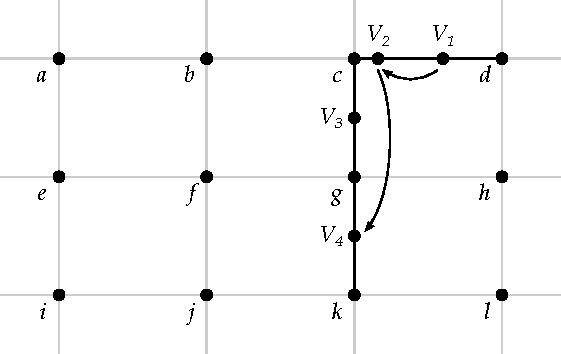
\includegraphics{ruta_siguiente_salto_4}
\decoRule
\caption[Selección del siguiente salto en ruta sin secuencia de varias aristas
con línea de visión]{Selección del siguiente salto en ruta sin secuencia de
varias aristas con línea de visión.}
\label{fig:ruta_siguiente_salto_4}
\end{figure}

Otro escenario es cuando un mensaje tiene que pasar de una subred a otra. En la
figura \ref{fig:siguiente_salto_cambio_subred} se muestra el grafo vial de dos
subredes vecinas. Los vehículos $V_1$ y $V_2$ forman parte de la subred 1, y
los vehículos $V_3$ y $V_4$ de la subred 2. El vehículo $V_1$ tiene un paquete
que debe retransmitir a la subred 2. Como el vértice $h$ es un vértice
\textit{gateway}, las aristas $\{i,h\}$ y $\{h,g\}$ son aristas
\textit{gateway}. Los vehículos que circulan por estas forman parte de ambas
subredes en ese momento, como se explicó en la sección \ref{sec:cambio_subred}.
En este caso, el vehículo $V_1$ selecciona aleatoriamente como siguiente salto
un vehículo vecino que se encuentre en la subred 2, que es el vehículo $V_3$ en
el ejemplo. Una vez que el vehículo $V_3$ recibe el paquete, comienza un
proceso de enrutamiento intrarregión dentro de la subred 2, en el que el paquete
debe llegar a su destino, si este se encuentra en la misma subred, o a la
siguiente subred.

\begin{figure}[th!]
\centering
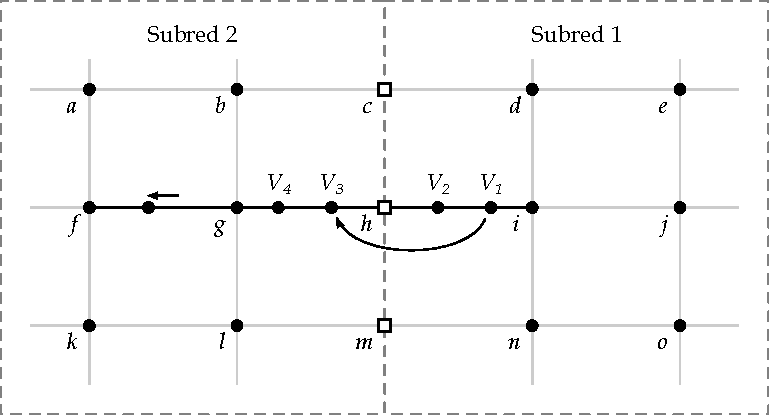
\includegraphics{siguiente_salto_cambio_subred}
\decoRule
\caption[Selección del siguiente salto en ruta sin secuencia de varias aristas
con línea de visión]{Selección del siguiente salto en ruta sin secuencia de
varias aristas con línea de visión.}
\label{fig:siguiente_salto_cambio_subred}
\end{figure}

\begin{algorithm}[th!]
\small
\caption{Selección del siguiente salto}
\label{alg:seleccion_siguiente_salto}
\DontPrintSemicolon
\LinesNumbered
    \KwData{$paquete$: Paquete a enrutar}
    \Begin{
        
    }
\end{algorithm}

\begin{algorithm}[th!]
\small
\caption{Enrutamiento de paquetes}
\label{alg:enrutar_paquete}
\DontPrintSemicolon
\LinesNumbered
    \KwData{$paquete$: Paquete a enrutar}
    \Begin{
        \If{$ValidarCabeceraPaquete(paquete) = Falso$}{
            descartar $paquete$ \;
        }
        $verticeDestinoLocal \gets ObtenerVerticeDestinoLocal(paquete)$ \;
    }
\end{algorithm}

%-----------------------------------
%   PARÁMETROS DE CONFIGURACIÓN
%-----------------------------------
\section{Parámetros de configuración}

\label{sec:parametros_configuracion}

\keyword{INTERVALO\_ANC\_VEHIC} --

\keyword{VIGENCIA\_VEHICULO\_VECINO} --

\keyword{INTERVALO\_ANC\_HOST} --

\keyword{VIGENCIA\_HOST\_VECINO} --

\keyword{ESPERA\_PONG} --

\keyword{VIGENCIA\_ARISTA\_ACTIVA} --

\keyword{VIGENCIA\_ARISTA\_INACTIVA} --

\keyword{VIGENCIA\_RUTA} --

\keyword{RADIO\_CERCANIA\_VERTICE} --
